%! Author = charon
%! Date = 6/4/24

\section{Hintergrund}\label{sec:hintergrund}
Folgendes Kapitel beschreibt die Grundlagen der in dieser Arbeit angewendeten Testing-Methoden und Herangehensweisen.
Hierfür werden zunächst die Software-Testing-Methoden vorgestellt, die im Applikations- und System-Testing verwendet werden.
Anschließend wird das Fuzzing als eine der wichtigsten Methoden des Software-Testings vorgestellt und kategorisiert.
Zum weiteren Verständnis werden die Grundlagen des \gls{tcp}-Protokolls erläutert.
Darauf aufbauend werden die Grundlagen des \gls{zup}s \gls{mqtt} vorgestellt und die Funktionsweise des Protokolls erläutert,
um eine ausreichende Grundlage zum Verständnis der Analyse zu schaffen.
%! Author = charon
%! Date = 6/4/24

\subsection{Software-Testing Methoden}\label{subsec:software-testing-methoden}
Das Fuzzing ist eine Software-Testing Methode zum Finden von Bugs und Sicherheitslücken in Applikationen.
Es gibt verschiedene Arten von Software-Testing Methoden, die in der Software-Entwicklung eingesetzt werden.
Die drei Kategorien sind White-Box, Black-Box und Grey-Box Testing.
Sie unterscheiden sich in der Art und Weise, wie sie die Software testen.
Jede Methode hat ihre eigenen Vor- und Nachteile und wird in verschiedenen Situationen eingesetzt.
In den folgenden Abschnitten werden die verschiedenen Software-Testing Methoden genauer erläutert.
\subsubsection{White-Box testing}\label{subsubsec:white-box-testing}
Es handelt sich um White-Box Testing, wenn der Tester Zugriff auf den Quellcode der Software hat.
Diese Testingmethode wird auch als \textit{Clear-Box}, \textit{Transparent-Box} oder \textit{Open-Box} Testing bezeichnet.
Der Tester kann den Quellcode der Software analysieren und die Testfälle basierend auf dem Quellcode erstellen~\cite{white-box-testing}.
White-Box Testing wird normalerweise von Entwicklern durchgeführt, um sicherzustellen, dass der Code korrekt funktioniert und keine Fehler enthält.
Es wird auch verwendet, um die Testabdeckung zu messen und sicherzustellen, dass alle Teile des Codes getestet wurden.
White-Box Testing ist eine sehr effektive Methode, um Fehler in der Software zu finden,
aber es erfordert auch eine gründliche Kenntnis des Quellcodes und der Software-Architektur.
Zu White-Box Testing gehören mitunter das \textit{Unit Testing}, bei dem einzelne Komponenten der Software getestet werden
und \textit{Path Testing} bei dem alle möglichen Programmpfade innerhalb eines zu testenden Abschnittes abgelaufen und überprüft werden sollen.\newline
Der Vorteil dieser Testmethode besteht darin, dass hierbei komplexe und auch strukturelle Fehler aufgedeckt werden können.
Die Anwendung einer solchen Testmethode findet im optimalen Fall während der Entwicklung einer Anwendung statt.
\subsubsection{Black-Box testing}\label{subsubsec:black-box-testing}
Bei Black-Box Testing wird kein Zugriff auf den Quellcode und die interne Struktur der Application gebraucht.
Das Ziel dieser Testmethode ist es zunächst mögliche Eingaben von Benutzern einer Software nachzuahmen~\cite{black-box-testing}.
Somit werden funktionalitäten einer Software getestet, ohne dass der Tester den Quellcode kennt.
In der Regel werden hierbei nur bereits kompilierte Software-Module oder von außen Zugreifbare Endpunkte getestet.
Anwendungsfälle einer solchen Herangehensweise entsprechen einem Penetrationstest oder eines Usability-Tests.
Der Vorteil von Black-Box Testing besteht darin, dass das \gls{zup} aus der Sicht des Answers getestet wird.
Dabei wird die Software auf ihre Funktionalität und Benutzerfreundlichkeit getestet.
\newline
Black-Box Testing ist eine effektive Methode, um sicherzustellen, dass die Software den gestellten Anforderungen
entspricht und keine offensichtlichen Fehler enthält.
Es ist jedoch schwierig, komplexe Fehler zu finden, da der Tester keinen Zugriff auf den Quellcode hat und nicht weiß,
wie die Software intern funktioniert.
\subsubsection{Grey-Box testing}\label{subsubsec:grey-box-testing}
Grey-Box Testing kombiniert beide Aspekte der bereits genannten Ansätze.
Hierbei werden Teile des \gls{zup} offengelegt.
Während beim White-Box Testing die interne Struktur oder der Code des Systems bekannt und getestet wird und beim Black-Box
Testing nur die externen Funktionalitäten ohne Wissen über den internen Aufbau geprüft werden,
ermöglicht Grey-Box Testing eine Balance zwischen diesen Ansätzen.
Beim Grey-Box Testing hat der Tester teilweise Kenntnisse über die interne Struktur der Anwendung oder des Systems,
verwendet diese Informationen jedoch hauptsächlich, um die Erstellung und Durchführung von Testszenarien zu optimieren,
die auf der Benutzeroberfläche basieren~\cite{Coulter2001GrayboxST}.
Diese Methode erlaubt es, gezielte Testfälle zu entwerfen, die nicht nur auf den sichtbaren Eingaben und Ausgaben basieren,
sondern auch auf dem Wissen über die zugrundeliegenden Datenflüsse, Algorithmen oder architektonischen Schwächen.
Grey-Box Testing wird häufig in Szenarien eingesetzt, in denen eine vollständige Kenntnis der internen Struktur nicht
notwendig oder verfügbar ist, jedoch ein gewisses Maß an Verständnis über die Architektur oder den Code notwendig ist,
um tiefere Testfälle zu entwickeln.
Diese Technik kann besonders nützlich sein bei der Validierung von Sicherheitsaspekten, der Integrationstests von komplexen
Systemen oder der Optimierung der Testabdeckung bei großen Anwendungen.
In der Praxis findet Grey-Box Testing Anwendung in Bereichen wie Web-Applikationen, APIs und bei sicherheitskritischen
Systemen, bei denen sowohl die Funktionalität als auch die interne Verarbeitung zuverlässig und sicher getestet werden müssen.
Die Methode bietet somit eine ausgewogene Teststrategie, die die Vorteile von White-Box und Black-Box Testing vereint,
um eine effektivere Fehlererkennung zu ermöglichen.
%! Author = charon
%! Date = 2/1/24

\subsection{Fuzzing}\label{subsec:fuzzing}
Fuzzing ist eine Black Box Testmethode, die darauf abzielt, Fehler in Software zu finden, indem zufällige oder
semi-zufällige Daten als Eingabe verwendet werden~\cite{fuzzing}.
Diese Daten werden in der Regel von einem Fuzzer generiert, der die Software mit den Daten füttert und auf unerwartetes Verhalten prüft.
Fuzzing ist eine effektive Methode, um Fehler in Software zu finden, die durch unerwartete Eingaben verursacht werden.
Es ist eine weit verbreitete Methode, um Sicherheitslücken in Software zu finden, die von Hackern ausgenutzt werden können.
Fuzzing kann auch dazu verwendet werden, um die Stabilität und Zuverlässigkeit von Software zu testen und um sicherzustellen,
dass sie korrekt funktioniert. \\
Es gibt verschiedene Arten von Fuzzern, die unterschiedliche Strategien und Techniken verwenden, um Fehler in Software zu finden.
Die Implementierung der Techniken und Strategien hängen von den Anforderungen und Zielen des Fuzzers ab.
In den folgenden Abschnitten werden die verschiedenen Arten von Fuzzern, ihre Strategien und Techniken näher erläutert.
%! Author = charon
%! Date = 5/23/24

\subsubsection{Arten des Fuzzing}\label{subsubsec:arten-des-fuzzing}
Trotz dem, dass Fuzzing als eine Black-Box Testmethode gilt, gibt es verschiedene Arten von Fuzzing, die unterschiedliche
Strategien und Techniken verwenden, um Fehler in Software zu finden.
Die Arten des Fuzzing sind somit in drei Kategorien unterteilt~\cite{iot-fuzzing}:
\begin{itemize}
    \item Black-box Fuzzing
    \item White-box Fuzzing
    \item Grey-box Fuzzing
\end{itemize}
Jede Kategorie hat ihre eigenen Vor- und Nachteile und wird in den folgenden Abschnitten näher erläutert.\newline
Im Black-box Fuzzing wird die Software ohne Kenntnis des ursprünglichen Quellcodes getestet.
Der Fuzzer generiert zufällige oder semi-zufällige Eingaben und übergibt sie der Software.
Das Generieren der Eingaben erfolgt in der Regel durch Mutation von vorhandenen Eingaben oder durch Generierung neuer Eingaben
und wird durch Regeln limitiert.
Mit diesen Regeln wird sichergestellt, dass die Mehrheit der Eingaben nicht von der zu untersuchenden Software -- aufgrund
von bspw.\ Syntaxfehlern -- abgelehnt wird.
Bei der Durchführung des Fuzzing überwacht der Fuzzer das Verhalten der Software und prüft, ob unerwartetes Verhalten auftritt. \\
Das Paradigma, das hierbei verfolgt wird, ist das Testen der Software ohne Kenntnis des Quellcodes, des Kontrollflusses und somit der internen
Logik, um die Benutzung aus der Perspektive eines Nutzers der Software nachzustellen.\\
Die Vorteile dieser Herangehensweise sind, dass der Code nicht verfügbar sein muss und somit auch proprietäre Software getestet werden kann.
Zudem werden Fehler gefunden, welche durch einen Nutzer der Software ausgelöst werden können.
Der ausschlaggebende Nachteil dieser Vorgehensweise ist, dass die Eingaben aufgrund limitierter Informationen über die Software
nur erschwert zu komplexeren Bugs führen können.
Das hat zufolge, dass die gefundenen Bugs meistens einfacher Natur sind und Eingaben oftmals nicht in tiefe Verzweigungen des Codes
gelangen können~\cite{black-box-fuzzing}.\newline\newline
Im Gegensatz zum Black-box Fuzzing wird im White-box Fuzzing der Quellcode der Software benötigt.
Der Fuzzer generiert Eingaben, die auf der Analyse des Quellcodes basieren.
Dabei werden die Eingaben so generiert, dass sie die verschiedenen Pfade und Verzweigungen des Codes abdecken.
Das Ziel ist es, die Software mit Eingaben zu füttern, die potenzielle Fehler in den verschiedenen Teilen des Codes auslösen.
Durch die Kenntnis des Quellcodes kann der Fuzzer gezieltere Eingaben generieren und somit auch komplexere Fehler finden.
Der Vorteil dieser Methode ist, dass sie effektiver ist als Black-box Fuzzing, da sie gezieltere Eingaben generieren kann.
Sie kann auch dazu verwendet werden, um spezifische Teile des Codes zu testen und um sicherzustellen, dass sie korrekt funktionieren.
Der Nachteil dieser Methode ist, dass der Quellcode verfügbar sein muss, was bei proprietärer Software ein Problem darstellen kann.
Zudem kann das White-box Fuzzing aufgrund der Komplexität des Codes und der Anzahl der möglichen Pfade und Verzweigungen
sehr aufwendig sein~\cite{black-box-fuzzing}.\newline\newline
Grey-box Fuzzing ist eine Kombination aus Black-box und White-box Fuzzing.
Die Verwendung eines Gray-box Fuzzers erfordert keinen Zugriff auf Sourcecode, jedoch kann dieser optional verwendet werden.
Unter Verwendung des Quellcodes kann die Performance des Fuzzers verbessert werden, indem gezieltere Eingaben generiert werden.
Die Vorteile des Gray-box Fuzzing sind, dass es effektiver ist als Black-box Fuzzing, da es gezieltere Eingaben generieren kann.
Außerdem ermöglicht dieser Ansatz auch das Analysieren von proprietärer Software aufgrund dessen, dass der Quellcode nicht für das
Fuzzen von Software notwendig ist~\cite{grey-box-fuzzing}.
Die Herangehensweise des Grey-box Fuzzing ist ähnlich zu dem des Black-box Fuzzing.
Jedoch können vor dem Kompilieren des Quellcodes Instruktionen des Fuzzers eingefügt werden, um das Fuzzing zu verbessern.
Zudem wird unter bspw.\ \gls{afl} ein eigener Compiler verwendet, um Metadaten des Programms zu extrahieren und weitere
Instrumentierungsanweisungen in den Code zu injizieren~\cite{afl-instr}.
%! Author = charon
%! Date = 5/23/24
\subsubsection{Generierung von Input}\label{subsubsec:generierung-von-input}
Die Generierung von Input ist ein wichtiger Bestandteil des Fuzzing-Prozesses.
Hierbei unterscheiden sich die Fuzzer in ihrer Herangehensweise und den Techniken, die sie verwenden, um Eingaben zu generieren.
Die Generierung von Input kann auf verschiedene Arten erfolgen, die in den folgenden Abschnitten näher erläutert werden.\newline\newline
\textit{Generationsbasierende}~\cite{iot-fuzzing} Fuzzer generieren Eingaben, indem sie eine Menge von Eingaben in Epochen erstellen.
Jede Epoche wird als Generation bezeichnet.
Diese Eingaben basieren auf einem vom Anwender festgelegten Regelwerk.
Diese Herangehensweise des Generierens von Eingaben ist effektiv, um die Software mit Eingaben zu versorgen, welche nicht
bereits im Vorfeld von dem \gls{zup} als fehlerhaft befunden werden sollen.
Beispielsweise ist dies Vorteilhaft, wenn besonders komplexe Syntax des Input vonnöten ist.\newline\newline
\textit{Mutationsbasierende}~\cite{iot-fuzzing} Fuzzer generieren Eingaben, indem sie vorhandene Eingaben, welche bereits im Vorfeld definiert wurden, verändern.
Hierbei wird der Aufbau und die Struktur der Eingaben standardmäßig nicht berücksichtigt.
Diese Veränderung wird Mutation genannt und kann auf verschiedene Arten erfolgen.
Die Mutation kann beispielsweise durch das Hinzufügen, Entfernen oder Verändern von Bytes in der Eingabe erfolgen.
Um die Güte der neu generierten Eingaben zu bestimmen, wird die Code Coverage -- also die im Quellcode erreichte Tiefe --
analysiert.
Eingaben, die besonders viele Codesegmente erreichen werden als besonders gut gewertet und als bevorzugte Eingabe für
weitere Mutationen verwendet.

%! Author = charon
%! Date = 5/23/24

\subsubsection{Intelligenz von Fuzzern}\label{subsubsec:intelligenz-von-fuzzern}
Die Intelligenz verschiedener Fuzzer kann in zwei Kategorien~\cite{fuzzer-intelligence} unterteilt werden:
\begin{itemize}
    \item Brute-Force Fuzzer
    \item Intelligente Fuzzer
\end{itemize}
Zu den \textit{Brute-Force} Fuzzern gehören diejenigen, die das Feedback eines Programms nicht interpretieren.
Hierzu werden die Eingaben zufällig generiert und an das \gls{zup} übergeben.
Aufgrund dessen werden die Eingaben nicht auf ihre Gültigkeit oder Korrektheit überprüft.
Dumme Fuzzer sind in der Regel einfach zu implementieren und erfordern keine speziellen Kenntnisse über das \gls{zup}.
Sie sind jedoch weniger effektiv als intelligente Fuzzer~\cite{fuzzer-intelligence}, da sie keine Informationen über das Verhalten des Programms
sammeln und somit nicht in der Lage sind, gezieltere Eingaben zu generieren.
Ein Vorteil der Verwendung von dummen Fuzzern ist, dass sie in der Regel schneller sind als intelligente Fuzzer.
Das ist darauf zurückzuführen, dass aufgrund der nicht verwendeten Feedback-Schleife -- in der die Antworten des \gls{zup}
auf die Eingaben bewertet werden und anhand dessen eine passende Generierung der Eingaben gewählt wird --
die Eingaben schneller generiert werden können.\newline\newline
\noindent Intelligente Fuzzer adaptieren die Generierung der Eingaben anhand des Feedbacks.
Hierzu werden die Reaktion des Programms auf die Eingabe, die Anzahl der ausgeführten Instruktionen
oder die Anzahl der gefundenen Bugs analysiert.
Der Fokus der Analyse hängt von der Implementierung des Fuzzers ab.
Intelligente Fuzzer können das Verhalten des Programms überwachen und auf unerwartete Ereignisse reagieren~\cite{smart-fuzzing}.
Sie können auch Informationen über die Struktur des Programms sammeln und diese Informationen verwenden, um gezieltere Eingaben zu generieren.\newline
Intelligente Fuzzer sind in der Regel effektiver als dumme Fuzzer, da sie gezieltere Eingaben generieren können.
Sie sind jedoch auch komplexer zu implementieren und erfordern spezielle Kenntnisse über das \gls{zup}.

%! Author = charon
%! Date = 5/23/24
\subsubsection{Strategien von Fuzzern}\label{subsubsec:strategien-von-fuzzern}
Fuzzer können verschiedene Strategien verfolgen, um Eingaben zu generieren und das Verhalten der Software zu überwachen.
Die Strategien können in zwei Kategorien unterteilt~\cite{iot-fuzzing} werden:
\begin{itemize}
    \item Abdeckung von Codepfaden
    \item Zielgerichtetes Fuzzen
\end{itemize}
Bei dem zielgerichteten Fuzzen werden nur bestimmte Teile des Codes getestet.
Der Fuzzer generiert Eingaben, die auf bestimmten Kriterien basieren, um gezielt Fehler in diesen Teilen des Codes zu finden.
Zu den Kriterien gehören beispielsweise die Anzahl der ausgeführten Instruktionen, die Anzahl der gefundenen Bugs oder
die Reaktion des Programms auf die Eingabe.
Bei dieser Technik handelt es sich in der Regel um einen White-Box Fuzzer.
Um nur auf bestimmte Teile eines Programms zu fokussieren, wird der Quellcode benötigt~\cite{directed-greybox-fuzzing}.\newline\newline
Bei der Strategie der Codepfadabdeckung wird versucht, möglichst viele Pfade und Verzweigungen des Codes abzudecken.
Der Fuzzer generiert Eingaben, die verschiedene Pfade und Verzweigungen des Codes abdecken, um potenzielle Fehler in verschiedenen
Teilen des Codes zu finden.
Diese Technik wird in der Regel von Black- und Grey-Box Fuzzern verwendet, da sie keine Kenntnis des Quellcodes benötigen und sich
somit anderer Informationen bedienen müssen.
Die Codepfadabdeckung ist eine effektive Methode, um sicherzustellen, dass große Teile des Codes getestet wurden~\cite{iot-fuzzing}.
Somit ist es ebenso möglich besonders komplexe Bugs und Schwachstellen in einem System zu finden, da die Eingaben besonders
tief in den Programmcode gelangen.

%! Author = charon
%! Date = 6/20/24

\subsection{Grundlagen der TCP/IP-Kommunikation}\label{subsec:tcp/ip-kommunikation}
Die \gls{tcp}/\gls{ip}-Kommunikation ist ein Protokoll-Stack, der für die Kommunikation zwischen Computern verwendet wird.
Der Protokoll-Stack besteht aus zwei Schichten, dem \gls{tcp}- und dem \gls{ip}-Protokoll~\cite{tcp-ip}.
Das \gls{ip}-Protokoll ist für die Adressierung und das Routing von Datenpaketen zuständig.
Das \gls{tcp}-Protokoll ist für die zuverlässige Übertragung von Datenpaketen zuständig.
Die Kommunikation zwischen zwei Computern erfolgt über eine Verbindung, die durch eine \gls{ip}-Adresse und einen Port identifiziert wird.
Die \gls{ip}-Adresse identifiziert den Computer und der Port identifiziert den Dienst, der auf dem Computer ausgeführt wird.
Die Kommunikation erfolgt über eine Reihe von Datenpaketen, die zwischen den beiden Computern ausgetauscht werden.
Die Datenpakete enthalten Informationen über den Absender, den Empfänger, die Daten selbst und eine Prüfsumme,
die zur Überprüfung der Datenintegrität verwendet wird.
Die gesamte Kommunikation kann in drei Schritten: \textit{Verbindungsaufbau}, \textit{Datenübertragung} und \textit{Verbindungsabbau}
eingeteilt werden.
Der Verbindungsaufbau erfolgt in der Regel über eine Reihe von Schritten, die als \textit{Handshake} bezeichnet werden~\cite{tcp-handshake}.
Dieser Handshake besteht aus den drei Schritten \textit{SYN}, \textit{SYN-ACK} und \textit{ACK}.
Im Rahmen des Verbindungsaufbaus erfolgt die Verbindung sowie die Herstellung der Verbindung zwischen den beiden Computern.
Während der Datenübertragung erfolgt ein Austausch der Daten zwischen zwei Kommunikationspartnern.
Der Verbindungsabbau impliziert die Trennung der Verbindung.
Die Implementierung der \gls{tcp}/\gls{ip}-Kommunikation erfolgt in der Regel über die Socket-Programmierung.
Bei der Socket-Programmierung unter UNIX-Systemen hierzu die bereits im System implementierte Socket-API verwendet.
Die Socket-API stellt eine Reihe von Funktionen zur Verfügung, die es einem Programm ermöglichen, mit dem Netzwerk zu kommunizieren.
Sockets werden in der Regel als Datei-Handle dargestellt und können vom Kernel gelesen und geschrieben werden.
Diese Dateien sind in der Regel nicht im Namespace des Dateisystems abgelegt.
Metadaten der Sockets werden jedoch im Dateisystem abgelegt und können zu Analysezwecken von weiteren Programmen verwendet werden.
Diese Metadaten können im Dateisystem unter \textit{/proc/net/tcp}, \textit{/proc/net/tcp6} und unter im Verzeichnis
\textit{/proc/sys/net} eingesehen werden~\cite{tcp-manpage}.\newline
Der Gesamte Stack kann in vier Schichten unterteilt werden:
\begin{itemize}
    \item Anwendungsschicht
    \item Transportschicht
    \item Internetschicht
    \item Netzwerk-Interface-Schicht
\end{itemize}
Die Anwendungsschicht ist die oberste Schicht des Protokoll-Stacks und enthält die Anwendungen,
die die Kommunikation zwischen den Computern ermöglichen.
Zu dieser Schicht gehören die von einer Anwendung verwendeten Protokolle, wie z.B.\ \gls{http}, \gls{ftp}, \gls{dns} oder \gls{smtp},
mithilfe derer Daten über ein Netzwerk übertragen werden.
Die Funktion der zweiten Schicht des Protokoll-Stacks, der sogenannten Transportschicht, besteht in der Übertragung von Datenpaketen.
In dieser Schicht obliegt die zuverlässige Übertragung von Datenpaketen dem \gls{tcp}-Protokoll.
Die Internetschicht stellt die dritte Schicht des Protokoll-Stacks dar und ist für die Adressierung sowie das Routing von Datenpaketen zuständig.
In dieser Schicht obliegt dem \gls{ip}-Protokoll die Adressierung und das Routing von Datenpaketen.
Die Netzwerkschicht stellt die unterste Schicht des Protokoll-Stacks dar und ist für die Verbindung mit einem Netzwerk
sowie der dazugehörigen Hardware zuständig.\newline
In dieser Arbeit wird die Anwendungsschicht des Protokoll-Stacks analysiert.
%! Author = charon
%! Date = 8/8/24

\subsection{Grundlagen des Mosquitto MQTT-Brokers}\label{subsec:mosquitto-mqtt}
Mosquitto ist ein Open-Source-Message-Broker, der das \gls{mqtt}-Protokoll implementiert.
\gls{mqtt} ist ein Publish/Subscribe-Protokoll, das für Netzwerke mit geringer Bandbreite,
hoher Latenz oder unzuverlässigen Verbindungen entwickelt wurde.
Es wird häufig in der \gls{iot}-Kommunikation verwendet, um Daten zwischen Geräten, Sensoren und Anwendungen auszutauschen.
\gls{mqtt}, und damit auch Mosquitto, baut auf dem \gls{tcp}/\gls{ip}-Stack auf, was eine zuverlässige Datenübertragung zwischen Client und
Server gewährleistet.
\gls{tcp} sorgt dabei für eine gesicherte, verbindungsorientierte Kommunikation, bei der Datenpakete in der richtigen
Reihenfolge und fehlerfrei übertragen werden.
Diese Basis auf dem \gls{tcp}/\gls{ip}-Stack macht \gls{mqtt} zu einem robusten und weit verbreiteten Protokoll für den Einsatz
in vernetzten Umgebungen, insbesondere im \gls{iot}-Bereich.
Mosquitto bietet eine Möglichkeit, \gls{mqtt}-Nachrichten zwischen verschiedenen Clients zu vermitteln.
Der \gls{mqtt}-Broker ermöglicht es Clients, Nachrichten an bestimmte Themen (Topics) zu senden (Publish) und/oder zu
empfangen (Subscribe).
Durch seine geringe Overhead-Belastung und die Unterstützung für \gls{qos}-Ebenen, stellt Mosquitto eine zuverlässige
Lösung für die Kommunikation in verteilten Systemen dar.
Es bietet auch erweiterte Funktionen wie Authentifizierung, Verschlüsselung (\gls{tls}) und Integration mit anderen
Diensten.\newline
Das Protokoll \gls{mqtt} definiert drei Arten von Nachrichten~\cite{mqtt}:
\begin{itemize}
    \item \textbf{Publish:} Ein Client sendet eine Nachricht an einen Broker, die dieser an alle Abonnenten weiterleitet.
    \item \textbf{Subscribe:} Ein Client abonniert ein bestimmtes Thema (Topic), um Nachrichten zu empfangen, die von anderen
          Clients zu diesem Thema gesendet werden.
    \item \textbf{Unsubscribe:} Ein Client beendet das Abonnement eines Themas und empfängt keine weiteren Nachrichten zu
          diesem Thema.
\end{itemize}
Der erste Schritt in diesem Zustand ist das Starten des \gls{mqtt}-Brokers.
Der Broker dient als Vermittler für die Nachrichten, die zwischen verschiedenen \gls{mqtt}-Clients ausgetauscht werden.
Dieser Schritt ist entscheidend für den weiteren Betrieb des Systems.
Nach dem Starten des \gls{mqtt}-Brokers geht das System in den Initialisierungszustand über.
Hier wird die Netzwerkschnittstelle initialisiert, die für die Kommunikation über \gls{mqtt} erforderlich ist.
Diese Initialisierung stellt sicher, dass das System in der Lage ist, sich mit anderen Geräten im Netzwerk zu verbinden
und Nachrichten zu senden oder zu empfangen.
Nach erfolgreicher Initialisierung wechselt das System in den Zustand \textit{Listening}.
In diesem Zustand wartet das System entweder darauf, dass es eine \gls{mqtt}-Nachricht empfängt oder es ist in einem Leerlaufzustand (Idle).
Dieser Zustand ist zentral für das System, da hier die Hauptoperationen entweder initiiert oder beendet werden.
Wenn eine MQTT-Nachricht empfangen wird, wechselt das System in den Verarbeitungszustand.
In diesem Zustand werden die empfangenen Nachrichten verarbeitet, und es kann entweder eine Nachricht veröffentlicht oder
das System kann sich für ein neues Thema (Topic) abonnieren~\cite{mqtt-manpage}.
Sollte die Verarbeitung eine Veröffentlichung erfordern, geht das System in den Zustand \textit{Publishing} über.
In diesem Zustand wird die verarbeitete Nachricht an den entsprechenden \gls{mqtt}-Topic veröffentlicht, sodass andere
abonnierte Clients diese empfangen können.
Alternativ kann das System in den Zustand \textit{Subscribing} wechseln, wenn die Verarbeitung das Abonnieren eines neuen Topics erfordert.
Dieser Zustand ermöglicht es dem System, Nachrichten von einem neuen Thema zu empfangen.
Wenn keine Nachricht zur Verarbeitung vorliegt, bleibt das System im Leerlauf.
Dieser Zustand wird auch erreicht, wenn alle anstehenden Aufgaben erledigt sind und das System auf neue Nachrichten oder Befehle wartet.
Sobald ein Herunterfahren (Shutdown) angefordert wird, wechselt das System in den Zustand Terminating.
In diesem Zustand werden alle notwendigen Ressourcen aufgeräumt, um das System ordnungsgemäß zu beenden.
Der endgültige Zustand des Systems ist \textit{Stopped}.
Nachdem alle Ressourcen bereinigt wurden, ist das System inaktiv und bereit, vollständig heruntergefahren zu werden.\newline
Diese Nachrichten werden über das \gls{tcp}-Protokoll zwischen Client und Broker ausgetauscht.
Der Broker verfügt über eine interne Datenstruktur, die die Themen und die zugehörigen Abonnenten speichert.
Diese Speicherung und das Weiterreichen dieser N
achrichten kann in einer State Machine abgebildet werden.
\begin{figure}[H]
    \centering
    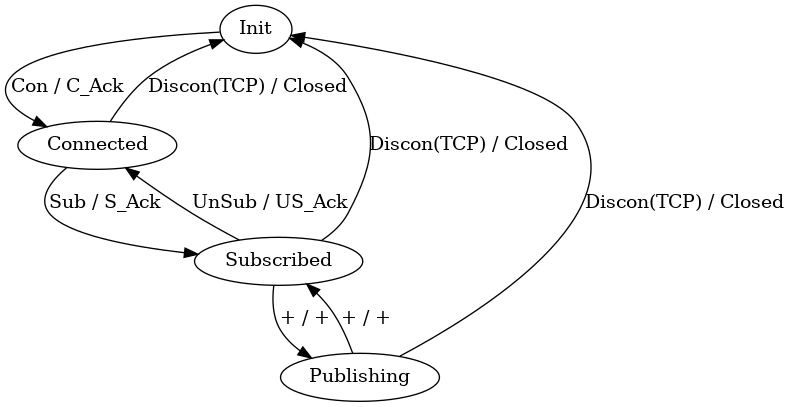
\includegraphics[width=\textwidth]{img/state_machine}
    \caption[State Machine des MQTT-Protokolls]{State Machine des Mosquitto MQTT-Protokolls. Sie beschreibt alle Zustände, die der Broker nach Empfangen von
    Nachrichten durchläuft. Beginnend mit der Überprüfung der Nachricht, über das Weiterleiten der Nachricht an die Abonnenten,
    bis hin zum Senden der Nachricht an die Clients.}
    \label{fig:mqtt_state_machine}
\end{figure}
\noindent Die Abbildung~\ref{fig:mqtt_state_machine} zeigt eine Zustandsmaschine (State Machine) für das \gls{mqtt}-Protokoll und beschreibt den Übergang zwischen
verschiedenen Verbindungszuständen eines \gls{mqtt}-Clients.
Diese Zustandsmaschine veranschaulicht, wie der \gls{mqtt}-Client in verschiedenen Situationen reagiert, z.B.\ beim Verbinden,
Abonnieren, Veröffentlichen und Trennen der Verbindung.\newline
Der Ausgangszustand der \gls{mqtt}-Zustandsmaschine ist der Init-Zustand.
Hier befindet sich der \gls{mqtt}-Client, bevor eine Verbindung zum Broker hergestellt wird oder nach einer Trennung.
Es ist der Ausgangspunkt und auch der Zustand, zu dem der Client nach einer Trennung zurückkehrt.
Wenn der Client eine Verbindung zum Broker herstellt (Con), wird ein Verbindungsbestätigungsnachricht (C\_Ack) empfangen
und der Zustand wechselt zu Connected.
Bei einer Trennung der \gls{tcp}-Verbindung (Discon(\gls{tcp})) wechselt der Zustand zu Closed.
In diesem Zustand ist der Client erfolgreich mit dem \gls{mqtt}-Broker verbunden.\newline
Der Client kann jetzt Abonnement- und Veröffentlichungsaktionen durchführen.
Der Client sendet eine Abonnementanfrage (Sub) an den Broker und erhält eine Bestätigungsnachricht (S\_Ack).
Der Zustand wechselt dann zu Subscribed.
Bei einer Trennung der \gls{tcp}-Verbindung (Discon(\gls{tcp})) wechselt der Zustand zu Closed.
In diesem Zustand hat der Client erfolgreich ein oder mehrere Themen (Topics) abonniert.
Der Client ist nun in der Lage, Nachrichten von den abonnierten Themen zu empfangen.
Der Client kann eine Nachricht veröffentlichen.\newline
Nach jedem erfolgreichen Veröffentlichungsprozess bleibt der Client im Subscribed-Zustand oder wechselt für die Veröffentlichung
kurzzeitig in den Publishing-Zustand.
Der Client kann eine Abmeldung (UnSub) von einem Thema anfordern und erhält eine Abmeldebestätigungsnachricht (US\_Ack).
Der Zustand kehrt dann zu Connected zurück.
Bei einer Trennung der \gls{tcp}-Verbindung (Discon(\gls{tcp})) wechselt der Zustand zu Closed.
In diesem Zustand veröffentlicht der Client Nachrichten an die abonnierten Themen.\newline
Es ist ein temporärer Zustand, in dem die Veröffentlichung von Nachrichten erfolgt.
Nach der Veröffentlichung einer Nachricht kehrt der Client in den Subscribed-Zustand zurück, um weitere Nachrichten empfangen zu können.
Bei einer Trennung der \gls{tcp}-Verbindung (Discon(\gls{tcp})) wechselt der Zustand zu Closed.\newline
Dies ist ein Endzustand, der erreicht wird, wenn die Verbindung zwischen dem Client und dem Broker getrennt wird.
Der Client ist nun nicht mehr in der Lage, Nachrichten zu senden oder zu empfangen.
Wenn der Client die Verbindung zum Broker wiederherstellt, kehrt der Zustand zu Init zurück, von wo aus er den Verbindungsprozess
neu starten kann.
\begin{figure}[H]
    \centering
    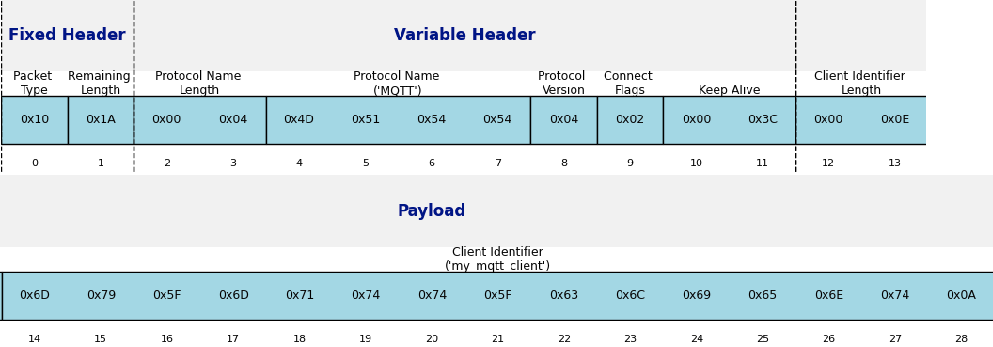
\includegraphics[width=\textwidth]{img/mqtt_packet_structure}
    \caption{Format einer \gls{mqtt}-Nachricht am beispiel eines Connect-Pakets.}
    \label{fig:mqtt_message_format}
\end{figure}
\noindent Die Struktur der zu sendenden Nachrichten ist von der verwendeten \gls{mqtt}-Version der Clients abhängig.
Die \gls{mqtt}-Version 3.1.1 -- die in dieser Arbeit verwendet wurde -- definiert ein festes Header-Format, das aus einem
Steuerbyte und einer variablen Länge besteht.
Als Nächstes folgt ein Variabler Header, der weitere Information über die Länge des Protokollnamens und den verwendeten
Protokollnamen, sowie die verwendete Protokollversion und ein Connect-Flag-Byte enthält.
das zehnte und elfte Byte enthalten die Keep-Alive-Zeit, die die maximale Zeit in Sekunden angibt, die der Client auf eine
Antwort des Brokers warten soll.
Die restlichen Bytes enthalten die Client-ID, die Länge des Benutzernamens und den Benutzernamen selbst, die
Länge des Passworts und das Passwort selbst.
Die \gls{mqtt}-Nachrichtenstruktur~\cite{mqtt} ist in Abbildung~\ref{fig:mqtt_message_format} dargestellt.
\newline
Die gesendeten Nachrichten haben im kürzesten Fall eine Länge von 2 Bytes, wobei das Steuerbyte für einen Verbindungsabbau
gesendet wird und somit nur aus dem Fixed-Header besteht.
Die Obergrenze der Größe eines validen Nachrichtenpakets beträgt 256 Megabytes~\cite{mqtt}.
%! Author = chaorn
%! Date = 06.09.24
\subsection{Verwendete Fuzzer}\label{subsec:verwendete-fuzzer}
In diesem Kapitel werden die in dieser Arbeit verwendeten Fuzzer vorgestellt.
Die Fuzzer \gls{afl}Net, boofuzz und Pulsar werden im Kontext der Performance-Analyse von Netzwerkfuzzern
verwendet und auf ihre Effektivität bei der Identifizierung von Schwachstellen in Netzwerkprotokollen untersucht.
Die Fuzzer boofuzz und \gls{afl}Net wurden in dieser Arbeit ausgewählt, da sie weit verbreitete Fuzzer mit umfangreicher
Dokumentation sind.
Pulsar wurde aufgrund seiner einzigartigen Fähigkeit, Netzwerkprotokolle zu erlernen und zu simulieren, ausgewählt.
Die Auswahl der drei Fuzzer ermöglicht es, verschiedene Ansätze und Techniken des Netzwerkfuzzings zu vergleichen und
einen möglichst umfassenden Einblick in die Herangehensweisen der Fuzzer zu erhalten.
\subsubsection{AFLNet}\label{subsubsec:aflnet}
\gls{afl} ist ein Fuzzer, der auf dem Prinzip der Codeabdeckung basiert.
Er zählt somit zu der Familie der Grey-Box Fuzzer und basiert auf einer mutationsbasierten Fuzzing-Technik.
Bei \gls{afl} handelt es sich ebenso um einen Applikationsfuzzer, welcher mithilfe eines Eingabestreams Daten
an ein \gls{zup} sendet und somit die Software auf Schwachstellen testet.\newline
Zur Analyse des Programms wird in dieser Arbeit jedoch ein Derivat von \gls{afl}(\gls{afl}Net) verwendet.
Es unterscheidet sich von dem ursprünglichen \gls{afl} dadurch, dass es speziell für die Analyse von Netzwerkprotokollen
entwickelt wurde.
Die Kernfunktionalität von \gls{afl} bleibt jedoch erhalten und wird um die Möglichkeit erweitert, Netzwerkprotokolle zu
analysieren.\newline
Hierzu müssen die Netzwerkpakete, die an das \gls{zup} gesendet werden, in einem speziellen Format vorliegen.
Die Extraktion der Netzwerkpakete erfolgt mithilfe eines \gls{pcap}-Dump-Files.
Diese Dump-Files enthalten den Netzwerkverkehr, der zwischen zwei Kommunikationspartnern stattgefunden hat.
Um diese Dump-Files zu generieren und somit den Netzwerkverkehr aufzunehmen wird das Tool \texttt{tcpdump} verwendet.
Zur Generierung der Netzwerkpakete wird das \gls{pcap}-Dump-File in ein \gls{afl}-kompatibles Format umgewandelt, indem
die rohen Datenflüsse extrahiert und in eine Datei geschrieben werden.
Die Extraktion der Datenflüsse kann mit Netzwerkanalyse-Tools wie \texttt{Wireshark} oder \texttt{tcpdump} erfolgen.
Hierzu wird im Repository von \gls{afl}Net~\cite{aflnet-repo} bereits eine Herangehensweise vorgestellt, wie die Datenflüsse mit
Wireshark extrahiert werden können.
Diese Datenflüsse werden dann als Bytestream von \gls{afl} als Eingabe verwendet, um das \gls{zup} zu fuzzen.
\begin{figure}[H]
    \centering
    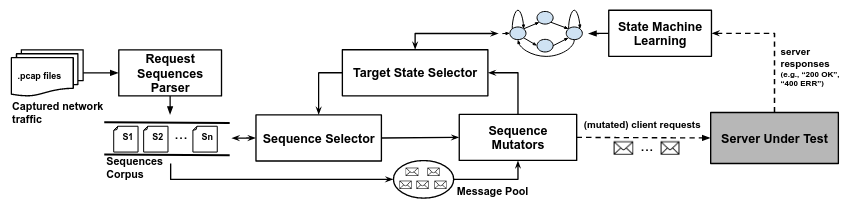
\includegraphics[width=\textwidth]{img/aflnet_arch}
    \caption[Architektur des AFLNet Fuzzers]{Die Abbildung zeigt die Architektur von \gls{afl}Net nach Pham Van-Thuan~\cite{AFLNet}.}
    \label{fig:aflnet_architecture}
\end{figure}
\noindent Zuerst muss das \gls{zup} gestartet und mir Eingaben gefüttert werden.
Während der Transaktion der Nachrichten wird der einhergehende Traffic mit einem Aufnahmeprogramm wie \texttt{tcpdump} aufgezeichnet.
Die aufgezeichneten Daten werden in ein \gls{pcap}-Dump-File geschrieben und müssen anschließend analysiert werden.
Dabei muss der Netzwerkverkehr in ein Format umgewandelt werden, das von \gls{afl}Net verstanden wird.
Dieses Format besteht in dem Fall dieser Arbeit aus einem Bytestream, der die Nachrichten des Netzwerkverkehrs enthält.
Die Nachrichten werden in einer Datei abgelegt und können dann von \gls{afl}Net als Eingabe verwendet werden.
Besonderes Augenmerk hierbei liegt auf der Analyse des Netzwerkverkehrs und der daraus resultierenden State Machine.
\gls{afl}Net analysiert den Netzwerkverkehr und extrahiert die Nachrichten, die zwischen Client und Server ausgetauscht werden.
Werden bei der Ausführung von Nachrichten bestimmte Zustände erreicht, so werden diese Zustände in einer State Machine
abgebildet und die State Machine mit dem neuen Zustand als Node erweitert.
Die State Machine wird mithilfe von \gls{afl}Net erlernt und ermöglicht es, den Zustand des \gls{zup} nachzuverfolgen.
Das Erlernen der State Machine erfolgt durch das Aufstellen eines Graphen, der die Zustände des \gls{zup} abbildet.
Hierbei werden die Zustände basierend auf den gesendeten Nachrichten und den vom \gls{zup} generierten Antworten identifiziert.
Dieser Graph wird initial bei der Testphase der Nachrichten erstellt und bei jeder neuen Nachricht erweitert.
Die Erweiterung des Graphen erfolgt durch das Hinzufügen von neuen Zuständen, die durch die Nachrichten erreicht werden~\cite{AFLNet}.
\newline
Anschließend werden die Nachrichten mit den enthaltenen Nachrichtensequenzen an einen in \gls{afl}Net implementierten
Sequence-Mutator übergeben.
Dieser Mutator generiert aus den gesendeten Nachrichten neue mutierte Nachrichten, die an das \gls{zup} übergeben werden
können.
\subsubsection{Boofuzz}\label{subsubsec:boofuzz}
Boofuzz ist ein Open-Source-Fuzzing-Framework, das zur automatisierten Sicherheitsprüfung von Software verwendet wird.
Es wurde als Fork des populären Sulley Fuzzing Frameworks entwickelt und bietet verbesserte Stabilität, erweiterte Funktionen
und aktive Wartung.
Boofuzz ist in Python geschrieben und ermöglicht das Erstellen von Fuzzing-Kampagnen durch die Definition von Testfällen,
die systematisch verschiedene Protokollfelder und Eingabeparameter abdecken.
Das Framework unterstützt sowohl Netzwerkprotokolle als auch dateibasierte Anwendungen, was es vielseitig einsetzbar macht.
Dabei kann es beispielsweise Protokolle wie HTTP, FTP oder Telnet fuzzen, um Schwachstellen in Netzwerkdiensten zu identifizieren.
Ein zentrales Merkmal von boofuzz ist seine Fähigkeit zur Überwachung des Zustands des Zielsystems während des Fuzzings.
Hierbei handelt es sich jedoch nicht um \textit{state-awareness} -- also den tatsächlich erreichten Zustand eines Programms --
sondern ob ein Dienst abgestürzt ist, und entsprechend reagieren, indem es den Testprozess anpasst oder erneut startet.
Da keine Informationen über den internen Zustand des Zielsystems benötigt werden und die Generierung der Eingaben
willkürlicher Natur ist, handelt es sich bei boofuzz um einen \textit{"Brute Force"} Black-Box-Fuzzer.
\subsubsection{Pulsar}\label{subsubsec:pulsar}
Pulsar ist ein Fuzzer und wird zu der Familie der Black-Box-Fuzzer gezählt.
Der Fuzzer wird dafür verwendet, um Internet Protokolle zu testen.
Er ermöglicht es, ohne jedweden Quellcode anhand von gesammelten Traffic-Dumps eine State Machine eines \gls{zup} zu erlernen.
Das Besondere an diesem Fuzzer ist, dass er anhand von gesammelten Daten ein Model trainiert,
welches es dem Untersucher des Programmes ermöglicht, das Programm zu simulieren und schlussendlich
gezielt zu fuzzen.
Bei der Simulation des Protokolls kann der Fuzzer sowohl die Rolle des Clients, als auch die Roller
des Servers einnehmen.
Gerade dieser Punkt ermöglicht es dem Untersucher des Programms große Flexibilität bei der Untersuchung zu erreichen.
Somit kann ein großer Teil des Programms untersucht werden und möglichst tief in die Struktur des \gls{zup} eingegriffen werden.
\newline
\noindent Das Training des Modells beruht auf der Analyse des eingefangenen Netzwerkverkehrs.
Dabei werden verschiedene Nachrichten von sowohl Client- als auch Serverseite auf Byte-Ebene untersucht und
ähnliche Strukturen extrahiert.
Die daraus extrahierten Nachrichtensequenzen werden darauffolgend in einen endlich-deterministischen Vektor abgebildet.
Die Zusammenkunft aus mehreren Vektoren ergibt ein Cluster.
Anhand der entstandenen Cluster wird eine approximierte Abbildung der State-Machine des Protokolls geschlussfolgert.
Bei der Erschließung der State Machine können die tatsächlichen Zustände nur teilweise erschlossen werden und ist somit
von der Güte des gesammelten Netzwerkverkehrs abhängig.
Der Netzwerkverkehr wird bei der Untersuchung von Pulsar annotiert, um die Nachrichten von Client und Server unterscheiden
zu können.
Zusammenhänge zwischen den Nachrichten werden anhand von bereits beobachteten Nachrichten erschlossen.
Diese werden in Tupeln miteinander verglichen und miteinander assoziiert.
Nachdem die Assoziation aller Mitteilungen abgeschlossen ist, besteht ein Markov Modell zweiter Ordnung.
Dieses Modell wird in einem Graphen abgebildet und kann somit als eine Annäherung der State Machine interpretiert werden.
Das Markov Modell wird im anschluss mit einem \gls{dfa} minimiert.
Der dabei entstandene \gls{dfa} erlaubt es Analysten die Zustände manuell untersuchen zu können und gegebenenfalls
die Zustände zu verfeinern und nachzuvollziehen~\cite{pulsar}.